\subsection{Method of Birth}
Methods of birth can be classified into 4 categories. They are:
\begin{enumerate}
    \item Cesarean section
    \item Vaginal (forceps)
    \item Vaginal (non-instrumental)
    \item Vaginal (vacuum)
\end{enumerate}
If we look at the overall data in Figure \ref{fig:method_au} of Australia we can see that as time passed all of these births of different methods are increasing but the number of vaginal birth has increased more over time in comparison with other methods.
\begin{figure}
  \centering
  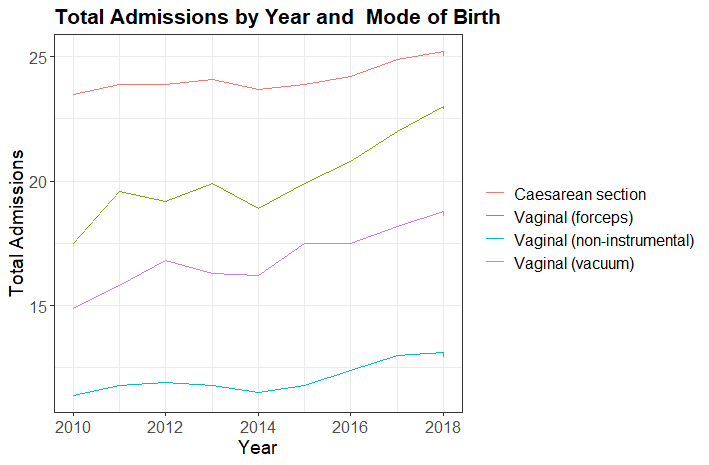
\includegraphics[width=0.75\textwidth]{subsections/method_of_birth/method_of_birth_au.png}
  \caption{Method of births in Australia over the years.}
  \label{fig:method_au}
\end{figure}
\subsubsection{Analysis: Onset Labour in ACT}
The onset of labor refers to the beginning of the active phase of labor, which is the process by which the uterus contracts and the cervix dilates to allow for the delivery of a baby. This is typically considered to occur when regular and frequent contractions begin, and the cervix starts to dilate and efface (thin out)\cite{birthColum}.

The onset of labor can vary from woman to woman and pregnancy to pregnancy. Some women may experience a gradual onset of contractions over several days, while others may have a sudden onset of strong and frequent contractions. The onset of labor can be influenced by a variety of factors, including hormones, fetal position, and maternal health. 

\begin{figure}
  \centering
  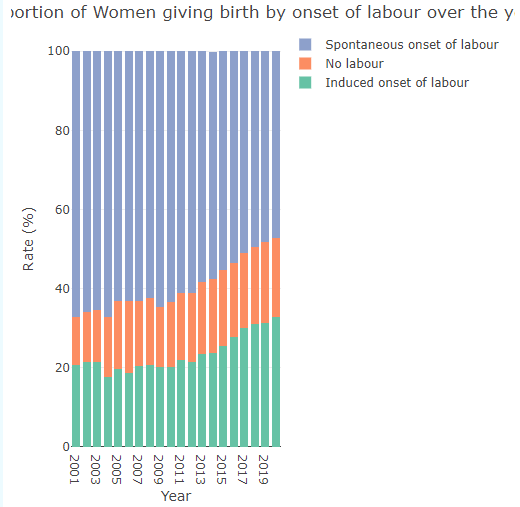
\includegraphics[width=0.45\textwidth]{subsections/method_of_birth/onset_method.png}
  \caption{Proportion of woman of ACT giving onset birth.}
  \label{fig:onset}
\end{figure}

\begin{figure}
  \centering
  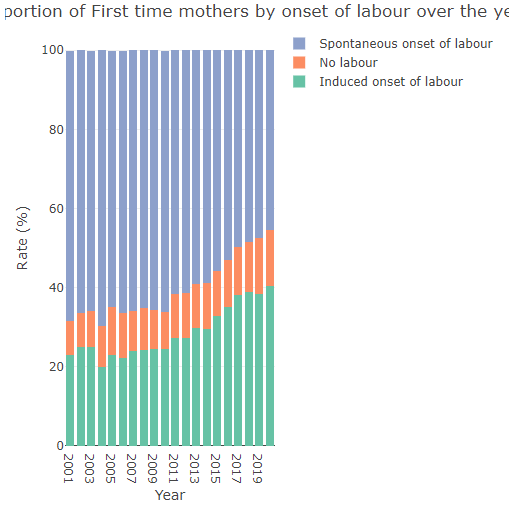
\includegraphics[width=0.45\textwidth]{subsections/method_of_birth/onset_method_first_time.png}
  \caption{Proportion of first-time mothers of ACT giving onset birth.}
  \label{fig:onsetFirsttime}
\end{figure}

To have a look at the data of mothers giving onset birth over the years we looked at the proportion and were curious to find out how the pattern changed. According to our observation, which is shown in Figures \ref{fig:onset} and \ref{fig:onsetFirsttime}, it is observed that spontaneous onset labour has decreased in last two decades while on the other hand, induced labour has increased over the years. We can see similar trends in the first-time mothers' data but the proportion of having no labour decreases significantly.
\subsubsection{Vaginal Births in ACT}
Vaginal birth, also known as normal vaginal delivery, is the natural way for a baby to be born through the birth canal. It offers several significant benefits for both the mother and the baby, including:

\begin{itemize}
  \item Quicker recovery: Vaginal birth typically has a shorter recovery time than a cesarean section, which is a surgical delivery. Mothers who have vaginal births can usually go home from the hospital sooner, and they often experience less pain and discomfort during the recovery period.
  \item Fewer complications: Vaginal birth is associated with fewer complications for both the mother and the baby compared to cesarean section. For example, the risk of infection, blood loss, and injury to internal organs is lower with vaginal birth.
  \item Better for breastfeeding: Babies who are born vaginally are more likely to have an easier time breastfeeding. This is because the pressure of passing through the birth canal helps to expel fluid from the baby's lungs and stimulates the release of hormones that help with breastfeeding.
  \item Improved gut health: Babies born vaginally also tend to have a healthier gut microbiome compared to those born via cesarean section. The bacteria that the baby is exposed to during vaginal birth can help to colonize the gut and support a healthy immune system.
  \item Psychological benefits: Some mothers report feeling a greater sense of empowerment and satisfaction after having a vaginal birth. This may be due to the sense of achievement and control that comes with delivering a baby without medical intervention.
\end{itemize}

Overall, vaginal birth is a safe and natural option for most women, and it offers several significant benefits for both the mother and the baby. However, it's important for each woman to discuss her individual medical history and pregnancy with her healthcare provider to determine the best course of action for her delivery.

We can see in figure \ref{fig:vaginal_act} Cesarean section method is more prominent among mothers who are over 40. Oppositely we can observe that younger women mostly have vaginal births. As the age increases the number of vaginal birth decreases and cesarean section increases.

\begin{figure}
  \centering
  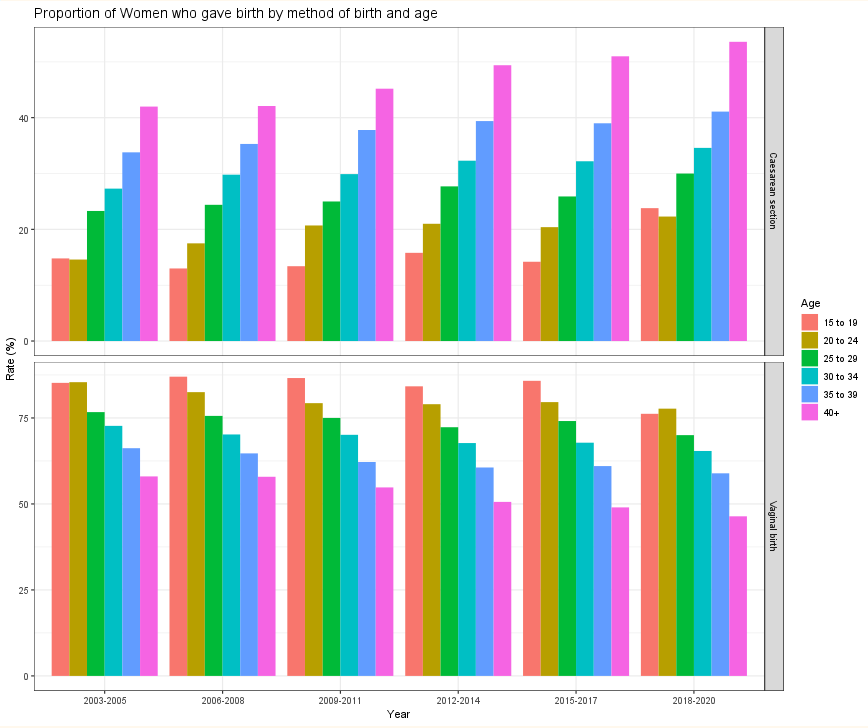
\includegraphics[width=1\textwidth]{subsections/method_of_birth/vagina_proportion.png}
  \caption{Different methods of birth in different mothers of different age groups (ACT).}
  \label{fig:vaginal_act}
\end{figure}